% academic work by Reza and Alireza Hosseini
% copyright (2015): Reza/Alireza Hosseini
% all this code was generated on authors own time
% authors did not receive any funding
% or were not employed at time of this work
% pdflatex ~/Dropbox/codes/academic/bike_sharing/latex/bike_sharing.tex
\documentclass[11pt,twoside,openany]{article}
\usepackage{
	amscd,
	amsbsy,
	amsfonts,
	amsmath,
	amssymb,
	booktabs,
	color,
	enumerate,
	float,
	graphics,
	graphicx,
	geometry,
	latexsym,
	multirow,
	natbib,
    subcaption,
	times,
	verbatim,
	xcolor}

%\usepackage[top=25mm, bottom=25mm, left=37.5mm, right=37.5mm]{geometry}
\graphicspath{
  {figs/}
  {figs/png/}
  {figs2/}
  {figs2/png/}
  {diagrams/}
  {emojis/}}

\newcommand{\E}{\mathop{{}\mathbb{E}}}
\newcommand{\var}{\text{Var}}
\newcommand{\bX}{{\bf X}}
\newcommand{\btX}{{\bf \tilde{X}}}
\newcommand{\btY}{{\bf \tilde{Y}}}
\newcommand{\bY}{{\bf Y}}
\newcommand{\bU}{{\bf U}}
\newcommand{\bZ}{{\bf Z}}
\newcommand{\bW}{{\bf W}}
\newcommand{\bWtilde}{{\bf \tilde{W}}}
\newcommand{\btW}{{\bf \tilde{W}}}
\newcommand{\tW}{{\tilde{W}}}
\newcommand{\bbeta}{{\bf \beta}}
\newcommand{\btheta}{{\bf \theta}}
\newcommand{\bPhi}{{\Phi}}
\newcommand{\bepsilon}{{\bf \epsilon}}
\newcommand{\bA}{{\bf A}}
\newcommand{\bphi}{{\bf \phi}}
\newcommand{\btau}{{\bf \tau}}
\newcommand{\bpsi}{{\bf \psi}}
\newcommand{\bPsi}{{\bf \Psi}}
\newcommand{\R}{\mathbb{R}}
\newcommand{\C}{\mathbb{C}}
\newcommand{\F}{\mathbb{F}}
\newcommand{\N}{\mathbb{N}}
\newcommand{\Z}{\mathbb{Z}}
\newcommand{\logit}{\mbox{logit}}
\setlength{\parindent}{12mm}
\setlength{\oddsidemargin}{12mm}
\setlength{\evensidemargin}{12mm}
\setlength{\topmargin}{-7mm}
\setlength{\textwidth}{150mm}
\newcommand{\QED}{\hspace*{\fill}\rule{2.5mm}{2.5mm}}
\newtheorem{theorem}{Theorem}[section]
\newtheorem{definition}{Definition}[section]
\renewcommand{\vec}[1]{\mbox{\boldmath $#1$}}
\newenvironment{proof}{\noindent{\bf Proof\ }}{\QED\\}
\newtheorem{proposition}{Proposition}[section]
\newtheorem{lemma}{Lemma}[section]
\newtheorem{hypothesis}{Hypothesis}[section]
\newtheorem{corollary}{Corollary}[section]
\renewcommand\floatpagefraction{.9}
\renewcommand\topfraction{.9}
\renewcommand\textfraction{.1}
\setcounter{totalnumber}{50}
\setcounter{topnumber}{50}
\setcounter{bottomnumber}{50}
\newcommand{\mysum}{\Sigma}


%\newtheorem{example}{Example}[section]
%\newenvironment{example}[1][Example]{\begin{trivlist}
\begin{document}
	\begin{center}
		{\large \bf Title}\\
		\vspace{0.1cm}
		{Alireza Hosseini$^{1}$, Reza Hosseini$^*$}\\
		{Yazd University}\\
		{\small Address$^{1,2}$: Yazd University, University Blvd. - Safayieh - Yazd}\\
		{$^1$email: arh31415@gmail.com, Corresponding author$^*$: reza1317@gmail.com}
	\end{center}


\begin{abstract}
\end{abstract}

\noindent {\bf Keywords:}
\section{Introduction}



\begin{figure}[H]
\centering
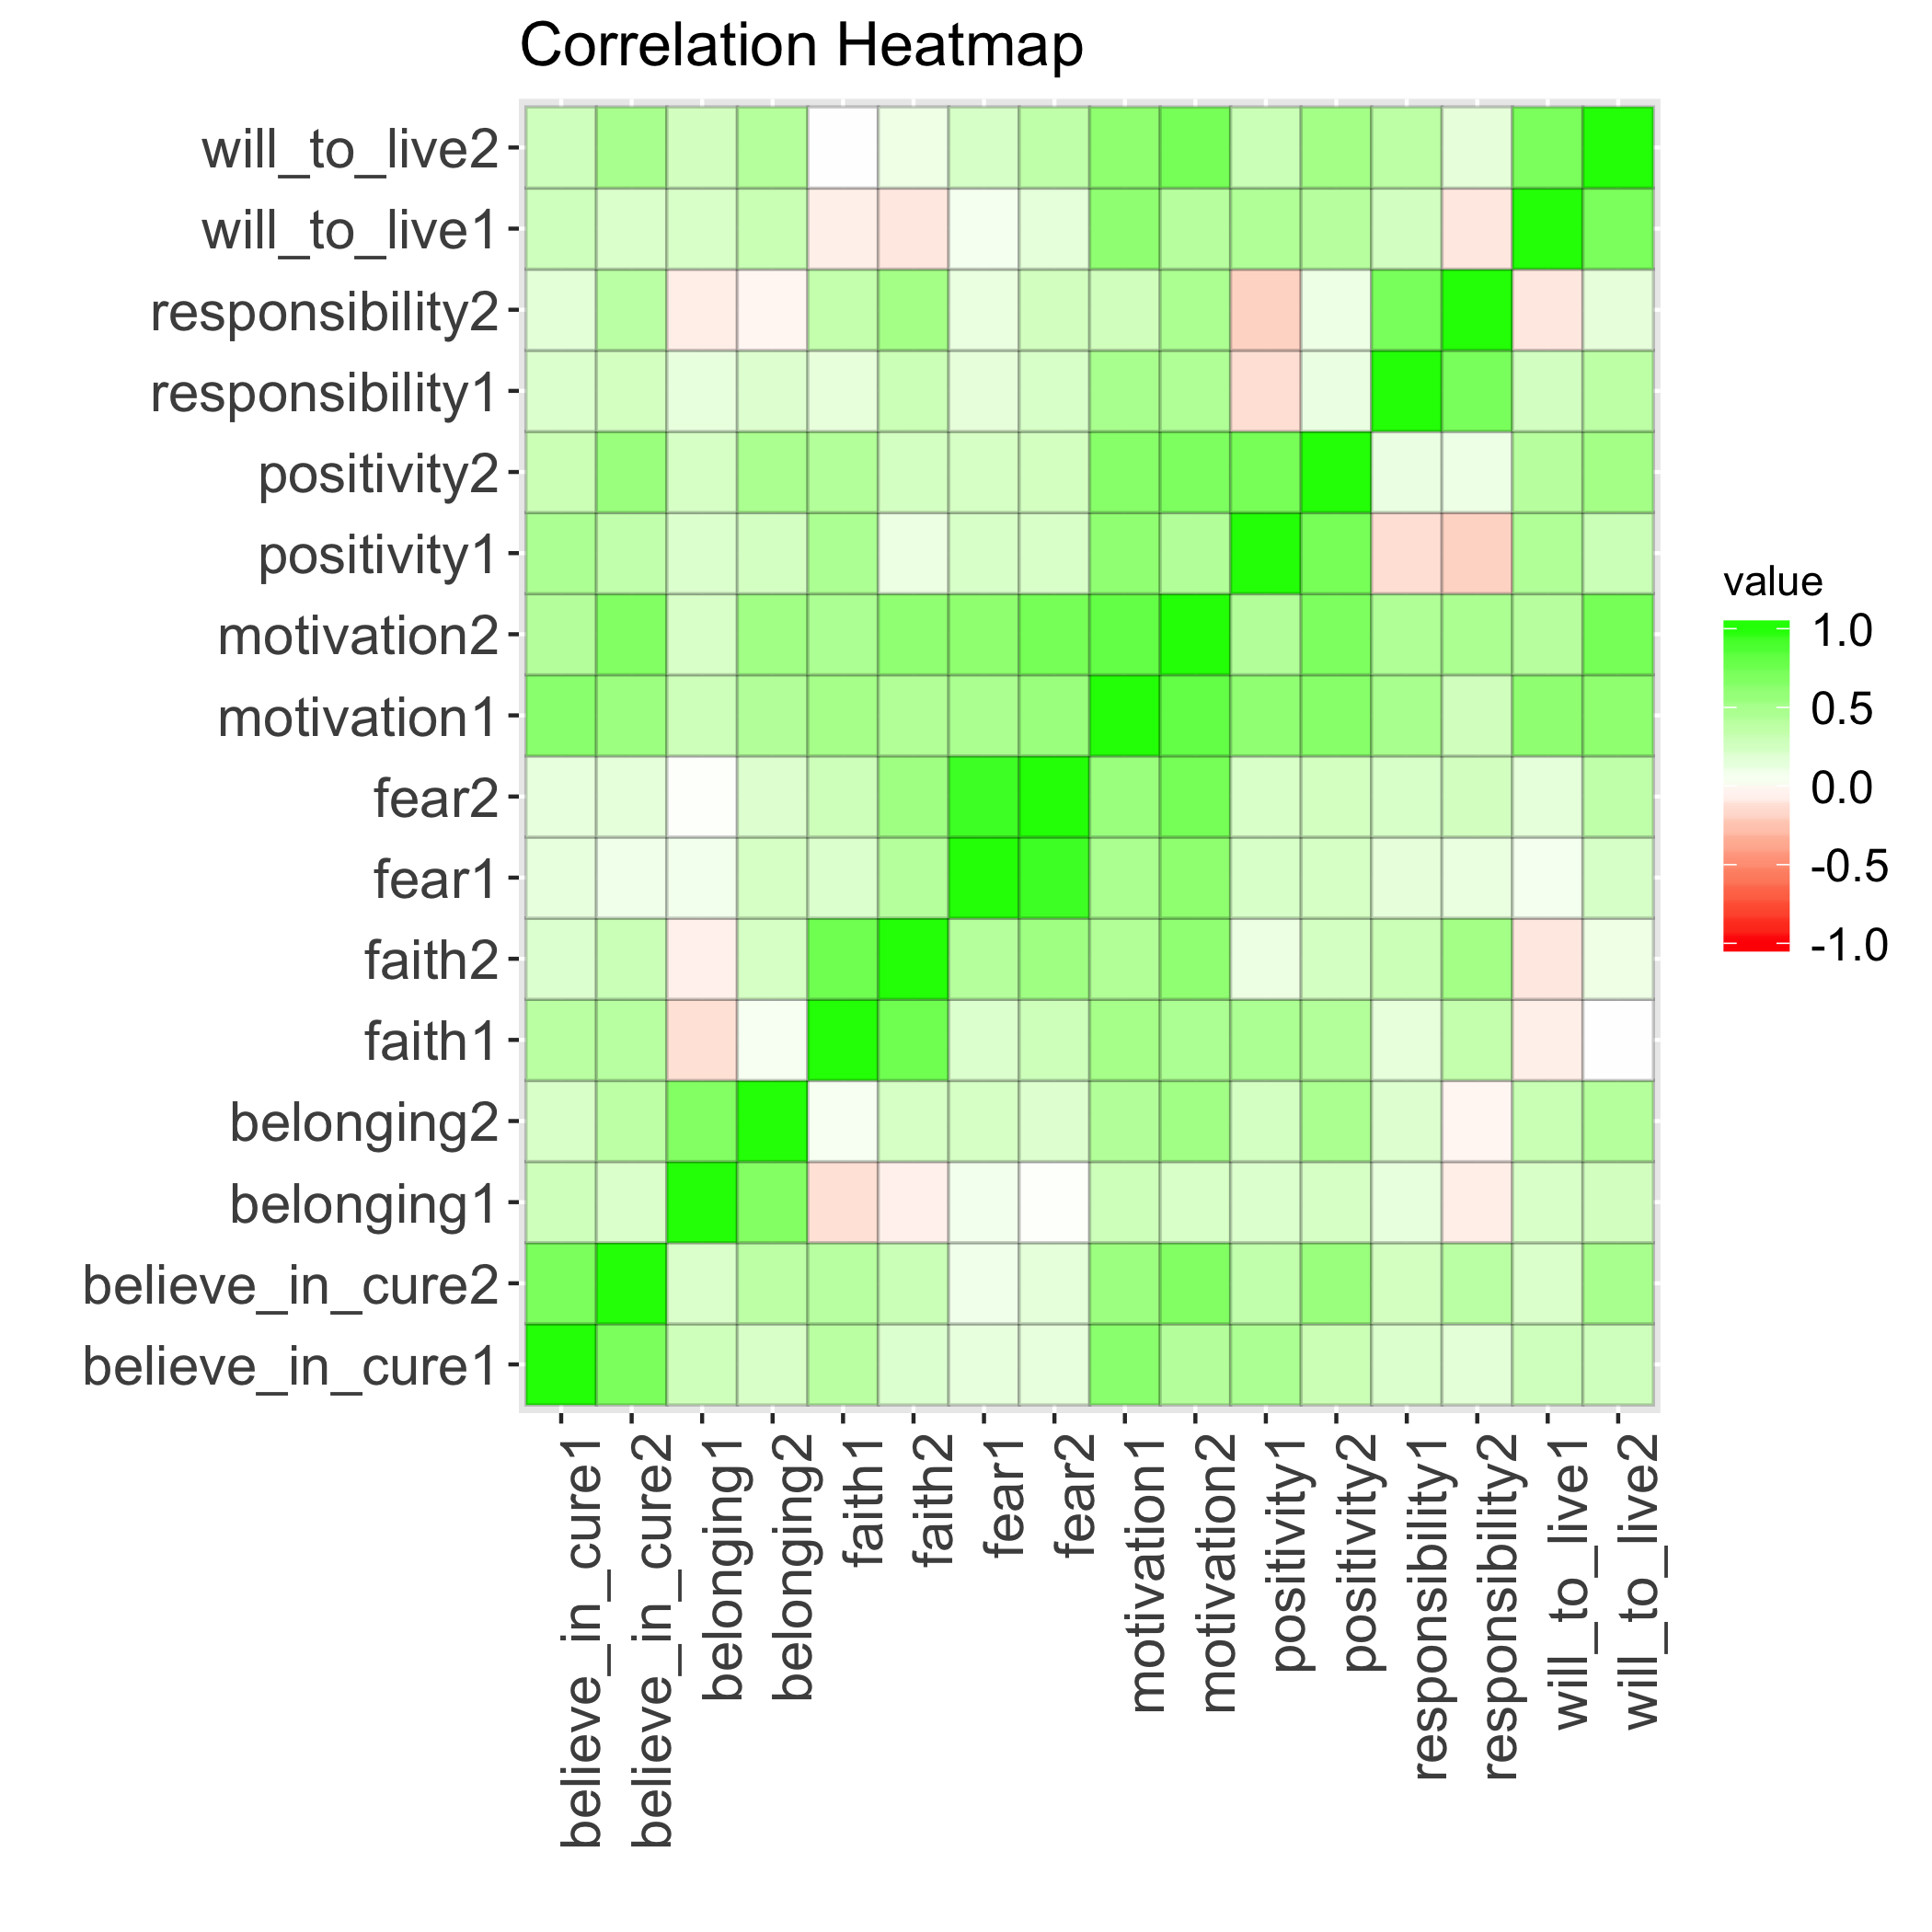
\includegraphics[width=0.5\linewidth]{correlation_over_time.png}
\caption{Correlation over time}
\label{correlation_over_time.png}
\end{figure}


\begin{figure}[H]
\centering
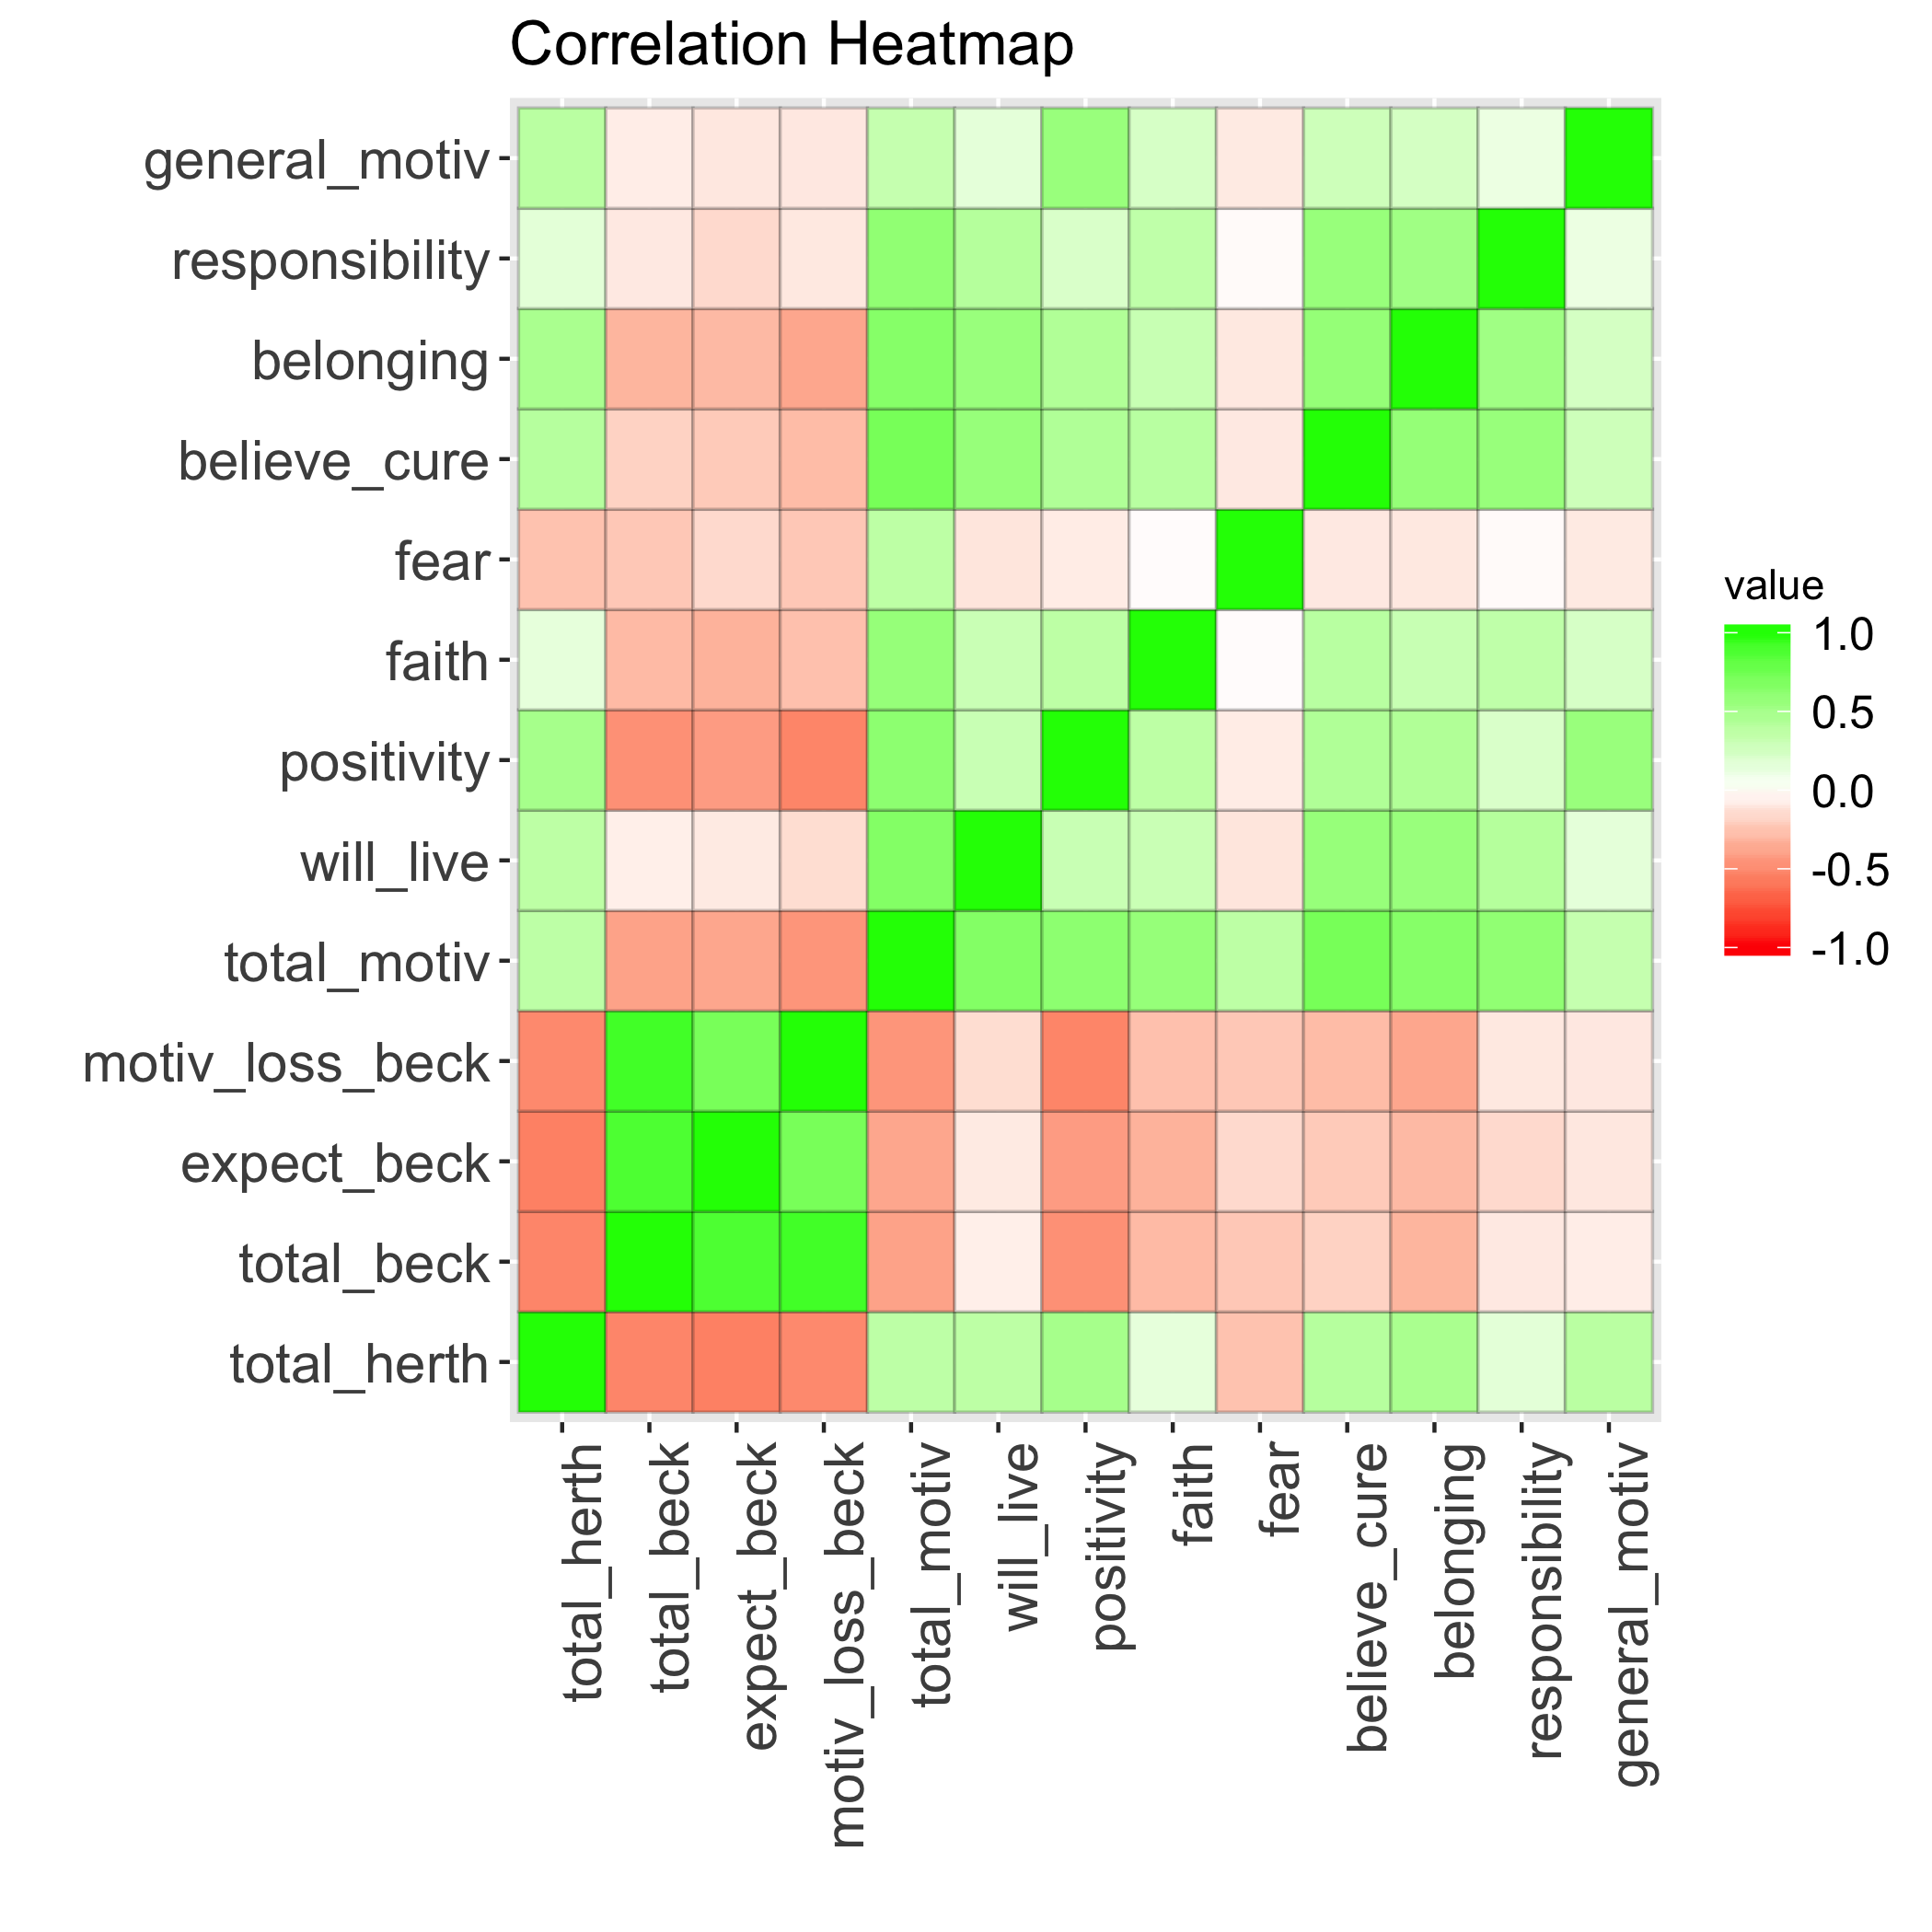
\includegraphics[width=0.5\linewidth]{correlation_across_aggregate_variables.png}
\caption{Correlation across aggregate variables}
\label{correlation_across_aggregate_variables.png}
\end{figure}


% latex table generated in R 3.6.0 by xtable 1.8-4 package
% Thu Dec 24 19:28:48 2020
\begin{table}[ht]
\centering
\begin{tabular}{|r|l|l|}
  \hline
 & Variable & Correlation.CI \\
  \hline
1 & believe\_in\_cure & 42, 86 \\
  2 & belonging & 36, 84 \\
  3 & faith & 51, 89 \\
  4 & fear & 85, 97 \\
  5 & motivation & 60, 91 \\
  6 & positivity & 45, 87 \\
  7 & responsibility & 43, 86 \\ 
  8 & will\_to\_live & 42, 86 \\
   \hline
\end{tabular}
\caption{Correlation over time}
\label{correlation_over_time}
\end{table}


\newpage]

\begin{table}[H] 
\tiny 
 \caption{Correlation conf interval across variables} 
 \label{correlation_conf_interval_across_variables} 
 \centering 
 \begin{adjustbox}{angle=270}  
 \begin{tabular} {|l|l|l|l|l|l|l|l|l|l|l|l|l|l|}  
 \hline 
  &  total\_herth & total\_beck & expect\_beck & motiv\_loss\_beck & total\_motiv & will\_live & positivity & faith & fear & believe\_cure & belonging & responsibility & general\_motiv \\ 
 \hline 
 total\_herth & {\color{green}100,100} & {\color{red}-62,-41} & {\color{red}-64,-44} & {\color{red}-60,-39} & {\color{green}25,49} & {\color{green}25,49} & {\color{green}38,59} & {\color{green}1,28} & {\color{red}-38,-12} & {\color{green}28,52} & {\color{green}36,57} & {\color{green}2,29} & {\color{green}27,50} \\ 
 \hline 
 total\_beck & {\color{red}-62,-41} & {\color{green}100,100} & {\color{green}83,92} & {\color{green}89,95} & {\color{red}-51,-27} & -21,7 & {\color{red}-57,-36} & {\color{red}-41,-16} & {\color{red}-36,-10} & {\color{red}-32,-5} & {\color{red}-43,-19} & -23,5 & -21,6 \\ 
 \hline 
 expect\_beck & {\color{red}-64,-44} & {\color{green}83,92} & {\color{green}100,100} & {\color{green}61,80} & {\color{red}-49,-26} & -23,5 & {\color{red}-53,-30} & {\color{red}-45,-20} & {\color{red}-29,-2} & {\color{red}-35,-9} & {\color{red}-42,-17} & {\color{red}-29,-2} & -23,4 \\ 
 \hline 
 motiv\_loss\_beck & {\color{red}-60,-39} & {\color{green}89,95} & {\color{green}61,80} & {\color{green}100,100} & {\color{red}-56,-34} & -27,0 & {\color{red}-62,-42} & {\color{red}-39,-13} & {\color{red}-36,-10} & {\color{red}-41,-15} & {\color{red}-49,-26} & -23,4 & -23,4 \\ 
 \hline 
 total\_motiv & {\color{green}25,49} & {\color{red}-51,-27} & {\color{red}-49,-26} & {\color{red}-56,-34} & {\color{green}100,100} & {\color{green}57,73} & {\color{green}52,69} & {\color{green}48,66} & {\color{green}25,49} & {\color{green}64,78} & {\color{green}56,72} & {\color{green}50,68} & {\color{green}20,45} \\ 
 \hline 
 will\_live & {\color{green}25,49} & -21,7 & -23,5 & -27,0 & {\color{green}57,73} & {\color{green}100,100} & {\color{green}18,43} & {\color{green}17,42} & -24,3 & {\color{green}47,65} & {\color{green}46,65} & {\color{green}29,52} & {\color{green}2,29} \\ 
 \hline 
 positivity & {\color{green}38,59} & {\color{red}-57,-36} & {\color{red}-53,-30} & {\color{red}-62,-42} & {\color{green}52,69} & {\color{green}18,43} & {\color{green}100,100} & {\color{green}25,49} & -21,6 & {\color{green}32,55} & {\color{green}32,54} & {\color{green}9,35} & {\color{green}45,65} \\ 
 \hline 
 faith & {\color{green}1,28} & {\color{red}-41,-16} & {\color{red}-45,-20} & {\color{red}-39,-13} & {\color{green}48,66} & {\color{green}17,42} & {\color{green}25,49} & {\color{green}100,100} & -15,12 & {\color{green}27,51} & {\color{green}19,44} & {\color{green}23,47} & {\color{green}10,36} \\ 
 \hline 
 fear & {\color{red}-38,-12} & {\color{red}-36,-10} & {\color{red}-29,-2} & {\color{red}-36,-10} & {\color{green}25,49} & -24,3 & -21,6 & -15,12 & {\color{green}100,100} & -23,5 & -23,4 & -16,12 & -22,5 \\ 
 \hline 
 believe\_cure & {\color{green}28,52} & {\color{red}-32,-5} & {\color{red}-35,-9} & {\color{red}-41,-15} & {\color{green}64,78} & {\color{green}47,65} & {\color{green}32,55} & {\color{green}27,51} & -23,5 & {\color{green}100,100} & {\color{green}48,66} & {\color{green}46,65} & {\color{green}16,41} \\ 
 \hline 
 belonging & {\color{green}36,57} & {\color{red}-43,-19} & {\color{red}-42,-17} & {\color{red}-49,-26} & {\color{green}56,72} & {\color{green}46,65} & {\color{green}32,54} & {\color{green}19,44} & -23,4 & {\color{green}48,66} & {\color{green}100,100} & {\color{green}42,62} & {\color{green}11,37} \\ 
 \hline 
 responsibility & {\color{green}2,29} & -23,5 & {\color{red}-29,-2} & -23,4 & {\color{green}50,68} & {\color{green}29,52} & {\color{green}9,35} & {\color{green}23,47} & -16,12 & {\color{green}46,65} & {\color{green}42,62} & {\color{green}100,100} & -2,25 \\ 
 \hline 
 general\_motiv & {\color{green}27,50} & -21,6 & -23,4 & -23,4 & {\color{green}20,45} & {\color{green}2,29} & {\color{green}45,65} & {\color{green}10,36} & -22,5 & {\color{green}16,41} & {\color{green}11,37} & -2,25 & {\color{green}100,100} \\ 
 \hline 
 \hline 
 \end{tabular} 
\end{adjustbox}  
\end{table} 

\begin{table}[H] 
\tiny 
 \caption{Correlation conf interval across variables} 
 \label{correlation_conf_interval_across_variables} 
 \centering 
 \begin{adjustbox}{angle=270}  
 \begin{tabular} {|l|l|l|l|l|l|l|l|l|l|l|l|l|l|}  
 \hline 
  &  total\_herth & total\_beck & expect\_beck & motiv\_loss\_beck & total\_motiv & will\_live & positivity & faith & fear & believe\_cure & belonging & responsibility & general\_motiv \\ 
 \hline 
 total\_herth & {\color{green}100,100} & {\color{red}-62,-41} & {\color{red}-64,-44} & {\color{red}-60,-39} & {\color{green}25,49} & {\color{green}25,49} & {\color{green}38,59} & {\color{green}1,28} & {\color{red}-38,-12} & {\color{green}28,52} & {\color{green}36,57} & {\color{green}2,29} & {\color{green}27,50} \\ 
 \hline 
 total\_beck & {\color{red}-62,-41} & {\color{green}100,100} & {\color{green}83,92} & {\color{green}89,95} & {\color{red}-51,-27} & -21,7 & {\color{red}-57,-36} & {\color{red}-41,-16} & {\color{red}-36,-10} & {\color{red}-32,-5} & {\color{red}-43,-19} & -23,5 & -21,6 \\ 
 \hline 
 expect\_beck & {\color{red}-64,-44} & {\color{green}83,92} & {\color{green}100,100} & {\color{green}61,80} & {\color{red}-49,-26} & -23,5 & {\color{red}-53,-30} & {\color{red}-45,-20} & {\color{red}-29,-2} & {\color{red}-35,-9} & {\color{red}-42,-17} & {\color{red}-29,-2} & -23,4 \\ 
 \hline 
 motiv\_loss\_beck & {\color{red}-60,-39} & {\color{green}89,95} & {\color{green}61,80} & {\color{green}100,100} & {\color{red}-56,-34} & -27,0 & {\color{red}-62,-42} & {\color{red}-39,-13} & {\color{red}-36,-10} & {\color{red}-41,-15} & {\color{red}-49,-26} & -23,4 & -23,4 \\ 
 \hline 
 total\_motiv & {\color{green}25,49} & {\color{red}-51,-27} & {\color{red}-49,-26} & {\color{red}-56,-34} & {\color{green}100,100} & {\color{green}57,73} & {\color{green}52,69} & {\color{green}48,66} & {\color{green}25,49} & {\color{green}64,78} & {\color{green}56,72} & {\color{green}50,68} & {\color{green}20,45} \\ 
 \hline 
 will\_live & {\color{green}25,49} & -21,7 & -23,5 & -27,0 & {\color{green}57,73} & {\color{green}100,100} & {\color{green}18,43} & {\color{green}17,42} & -24,3 & {\color{green}47,65} & {\color{green}46,65} & {\color{green}29,52} & {\color{green}2,29} \\ 
 \hline 
 positivity & {\color{green}38,59} & {\color{red}-57,-36} & {\color{red}-53,-30} & {\color{red}-62,-42} & {\color{green}52,69} & {\color{green}18,43} & {\color{green}100,100} & {\color{green}25,49} & -21,6 & {\color{green}32,55} & {\color{green}32,54} & {\color{green}9,35} & {\color{green}45,65} \\ 
 \hline 
 faith & {\color{green}1,28} & {\color{red}-41,-16} & {\color{red}-45,-20} & {\color{red}-39,-13} & {\color{green}48,66} & {\color{green}17,42} & {\color{green}25,49} & {\color{green}100,100} & -15,12 & {\color{green}27,51} & {\color{green}19,44} & {\color{green}23,47} & {\color{green}10,36} \\ 
 \hline 
 fear & {\color{red}-38,-12} & {\color{red}-36,-10} & {\color{red}-29,-2} & {\color{red}-36,-10} & {\color{green}25,49} & -24,3 & -21,6 & -15,12 & {\color{green}100,100} & -23,5 & -23,4 & -16,12 & -22,5 \\ 
 \hline 
 believe\_cure & {\color{green}28,52} & {\color{red}-32,-5} & {\color{red}-35,-9} & {\color{red}-41,-15} & {\color{green}64,78} & {\color{green}47,65} & {\color{green}32,55} & {\color{green}27,51} & -23,5 & {\color{green}100,100} & {\color{green}48,66} & {\color{green}46,65} & {\color{green}16,41} \\ 
 \hline 
 belonging & {\color{green}36,57} & {\color{red}-43,-19} & {\color{red}-42,-17} & {\color{red}-49,-26} & {\color{green}56,72} & {\color{green}46,65} & {\color{green}32,54} & {\color{green}19,44} & -23,4 & {\color{green}48,66} & {\color{green}100,100} & {\color{green}42,62} & {\color{green}11,37} \\ 
 \hline 
 responsibility & {\color{green}2,29} & -23,5 & {\color{red}-29,-2} & -23,4 & {\color{green}50,68} & {\color{green}29,52} & {\color{green}9,35} & {\color{green}23,47} & -16,12 & {\color{green}46,65} & {\color{green}42,62} & {\color{green}100,100} & -2,25 \\ 
 \hline 
 general\_motiv & {\color{green}27,50} & -21,6 & -23,4 & -23,4 & {\color{green}20,45} & {\color{green}2,29} & {\color{green}45,65} & {\color{green}10,36} & -22,5 & {\color{green}16,41} & {\color{green}11,37} & -2,25 & {\color{green}100,100} \\ 
 \hline 
 \hline 
 \end{tabular} 
\end{adjustbox}  
\end{table} 
 
\begin{table}[H] 
\tiny 
 \caption{Correlation conf interval across variables} 
 \label{correlation_conf_interval_across_variables} 
 \centering 
 \begin{adjustbox}{angle=270}  
 \begin{tabular} {|l|l|l|l|l|l|l|l|l|l|l|l|l|l|}  
 \hline 
  &  total\_herth & total\_beck & expect\_beck & motiv\_loss\_beck & total\_motiv & will\_live & positivity & faith & fear & believe\_cure & belonging & responsibility & general\_motiv \\ 
 \hline 
 total\_herth & {\color{green}100,100} & {\color{red}-62,-41} & {\color{red}-64,-44} & {\color{red}-60,-39} & {\color{green}25,49} & {\color{green}25,49} & {\color{green}38,59} & {\color{green}1,28} & {\color{red}-38,-12} & {\color{green}28,52} & {\color{green}36,57} & {\color{green}2,29} & {\color{green}27,50} \\ 
 \hline 
 total\_beck & {\color{red}-62,-41} & {\color{green}100,100} & {\color{green}83,92} & {\color{green}89,95} & {\color{red}-51,-27} & -21,7 & {\color{red}-57,-36} & {\color{red}-41,-16} & {\color{red}-36,-10} & {\color{red}-32,-5} & {\color{red}-43,-19} & -23,5 & -21,6 \\ 
 \hline 
 expect\_beck & {\color{red}-64,-44} & {\color{green}83,92} & {\color{green}100,100} & {\color{green}61,80} & {\color{red}-49,-26} & -23,5 & {\color{red}-53,-30} & {\color{red}-45,-20} & {\color{red}-29,-2} & {\color{red}-35,-9} & {\color{red}-42,-17} & {\color{red}-29,-2} & -23,4 \\ 
 \hline 
 motiv\_loss\_beck & {\color{red}-60,-39} & {\color{green}89,95} & {\color{green}61,80} & {\color{green}100,100} & {\color{red}-56,-34} & -27,0 & {\color{red}-62,-42} & {\color{red}-39,-13} & {\color{red}-36,-10} & {\color{red}-41,-15} & {\color{red}-49,-26} & -23,4 & -23,4 \\ 
 \hline 
 total\_motiv & {\color{green}25,49} & {\color{red}-51,-27} & {\color{red}-49,-26} & {\color{red}-56,-34} & {\color{green}100,100} & {\color{green}57,73} & {\color{green}52,69} & {\color{green}48,66} & {\color{green}25,49} & {\color{green}64,78} & {\color{green}56,72} & {\color{green}50,68} & {\color{green}20,45} \\ 
 \hline 
 will\_live & {\color{green}25,49} & -21,7 & -23,5 & -27,0 & {\color{green}57,73} & {\color{green}100,100} & {\color{green}18,43} & {\color{green}17,42} & -24,3 & {\color{green}47,65} & {\color{green}46,65} & {\color{green}29,52} & {\color{green}2,29} \\ 
 \hline 
 positivity & {\color{green}38,59} & {\color{red}-57,-36} & {\color{red}-53,-30} & {\color{red}-62,-42} & {\color{green}52,69} & {\color{green}18,43} & {\color{green}100,100} & {\color{green}25,49} & -21,6 & {\color{green}32,55} & {\color{green}32,54} & {\color{green}9,35} & {\color{green}45,65} \\ 
 \hline 
 faith & {\color{green}1,28} & {\color{red}-41,-16} & {\color{red}-45,-20} & {\color{red}-39,-13} & {\color{green}48,66} & {\color{green}17,42} & {\color{green}25,49} & {\color{green}100,100} & -15,12 & {\color{green}27,51} & {\color{green}19,44} & {\color{green}23,47} & {\color{green}10,36} \\ 
 \hline 
 fear & {\color{red}-38,-12} & {\color{red}-36,-10} & {\color{red}-29,-2} & {\color{red}-36,-10} & {\color{green}25,49} & -24,3 & -21,6 & -15,12 & {\color{green}100,100} & -23,5 & -23,4 & -16,12 & -22,5 \\ 
 \hline 
 believe\_cure & {\color{green}28,52} & {\color{red}-32,-5} & {\color{red}-35,-9} & {\color{red}-41,-15} & {\color{green}64,78} & {\color{green}47,65} & {\color{green}32,55} & {\color{green}27,51} & -23,5 & {\color{green}100,100} & {\color{green}48,66} & {\color{green}46,65} & {\color{green}16,41} \\ 
 \hline 
 belonging & {\color{green}36,57} & {\color{red}-43,-19} & {\color{red}-42,-17} & {\color{red}-49,-26} & {\color{green}56,72} & {\color{green}46,65} & {\color{green}32,54} & {\color{green}19,44} & -23,4 & {\color{green}48,66} & {\color{green}100,100} & {\color{green}42,62} & {\color{green}11,37} \\ 
 \hline 
 responsibility & {\color{green}2,29} & -23,5 & {\color{red}-29,-2} & -23,4 & {\color{green}50,68} & {\color{green}29,52} & {\color{green}9,35} & {\color{green}23,47} & -16,12 & {\color{green}46,65} & {\color{green}42,62} & {\color{green}100,100} & -2,25 \\ 
 \hline 
 general\_motiv & {\color{green}27,50} & -21,6 & -23,4 & -23,4 & {\color{green}20,45} & {\color{green}2,29} & {\color{green}45,65} & {\color{green}10,36} & -22,5 & {\color{green}16,41} & {\color{green}11,37} & -2,25 & {\color{green}100,100} \\ 
 \hline 
 \hline 
 \end{tabular} 
\end{adjustbox}  
\end{table} 
 



\vspace{2cm}
\noindent {\bf Acknowledgements.} Thanks.

\begin{thebibliography}{99}

\bibitem[Akaike (1974)]{akaike-1974}
Akaike, H. (1974)
\newblock A new look at the statistical model identification.
\newblock \emph{IEEE Transactions on Automatic Control}, AC-19:716--723.

%%% over-dispersion papers
\bibitem[Berk and MacDonald(2008)]{berk-2008}
Berk R. and MacDonald J. (2008)
\newblock Overdispersion and Poisson regression.
\newblock \emph{Journal of Quantitative Criminology}. 24(3):269--284. doi:10.1007/s10940--008--9048--4.

\bibitem[Efron(1986)]{efron-1986}
Efron, B. (1986)
\newblock Double exponential families and their use in generalized linear regression.
\newblock Journal of the American Statistical Association, 81:709--721.

\bibitem[Heinen(2003)]{heinen-2003}
Heinen A. (2003)
\newblock Modelling time series count data: an autoregressive conditional poisson model.
\newblock Center for Operations Research and Econometrics (CORE) Discussion Paper No. 2003--63,
University of Louvain, Belgium

%% end of over-dispersion papers

\bibitem[Fanaee et~al.(2013)]{fanaee-2013}
Fanaee-T, Hadi, and Gama, Joao (2013)
\newblock Event labeling combining ensemble detectors and background knowledge
\newblock \emph{Progress in Artificial Intelligence}, pp.\;1--15, Springer Berlin Heidelberg.

\bibitem[Fokianos(2012)]{fokianos-2012}
Fokianos, K.\;(2012)
\newblock Count Time Series Models
\newblock Handbook of Statistics, Volume 30, Chapter 12, pp.\;315--348
Time Series Analysis: Methods and Applications Edited by Rao, T.\;S., Rao, S.\;S. and Rao C.R.

\bibitem[Hastie et~al.(2009)]{hastie-2009}
Hastie, T., Tibshirani, R. and Friedman, J. H. (2009)
\newblock \emph{The Elements of Statistical Learning}, Second Edition.
\newblock Springer

\bibitem[Hosseini et~al.(2011a)]{hosseini-2011-categ}
Hosseini, R., Le, N.\;and Zidek, J. (2011a)
\newblock A Characterization of Categorical Markov Chains.
\newblock \emph{Journal of Statistical Theory and Practice}, 5(2):261--284

\bibitem[Hosseini et~al.(2011b)]{hosseini-bin-pcpn}
Hosseini, R., Le, N.\;and Zidek, J. (2011b)
\newblock Selecting a binary Markov model for a precipitation process.
\newblock \emph{Environmental and Ecological Statistics}, 18(4):795--820

\bibitem[R.\;Hosseini et~al.(2012)]{hosseini-bin-temp}
Hosseini, R., Le, N. and Zidek, J. (2012)
\newblock Time-Varying Markov Models for Binary Temperature Series in Agrorisk Management.
\newblock \emph{Journal of Agricultural Biological and Ecological Statistics},  17(2):283--305

\bibitem[Hosseini et~al.(2015a)]{hosseini-takemura-2015}
Hosseini, R., Takemura, A.\;and Hosseini, A.\;(2015a)
\newblock Non-linear time-varying stochastic models for agroclimate risk assessment.
\newblock \emph{Environmental and Ecological Statistics}, 22(2):227--246.

\bibitem[Hosseini et~al.(2015b)]{hosseini-RS-2015}
Hosseini, R., Newlands, N.\;K., Dean, C.\;B.\;and Takemura, A.\;(2015b)
\newblock Statistical modeling of soil moisture, integrating satellite remote-sensing (SAR) and ground-based data.
\newblock \emph{Remote Sensing}, 7(3):2752--2780

\bibitem[Hosseini et~al.(2017)]{hosseini-pcpn-2017}
Hosseini, A., Hosseini, R., Zare-Mehrjerdi and Y., Abooie M.\;H.\;(2017)
\newblock Capturing the time-dependence in the precipitation process for weather risk assessment.
\newblock \emph{Stochastic Environmental Research and Risk Assessment}, 31(3):609--627

\bibitem[Kedem et~al.(2002)]{kedem}
Kedem, B.\;and Fokianos, K.\;(2002)
\newblock \emph{Regression Models for Time Series Analysis},
\newblock Wiley Series in Probability and Statistics

\bibitem[Nastic et~al.(2012)]{nastic-2012}
Nastic, A.\;S.,  Ristic M.\;M. and Bakouch, H.\;S. (2012)
\newblock A combined geometric INAR(p) model based on negative binomial thinning
\newblock \emph{Mathematical and Computer Modelling} 55:1665--1672

%\bibitem[Paroli(2000)]{paroli-2000}
%Paroli R., Redaelli G.\;and Spezia L.\;(2000)
%\newblock Poisson hidden Markov models for time series of overdispersed insurance counts.
%\newblock ASTIN Colloquium International Actuarial Association- Brussels, Belgium, pp.\;461--474

\bibitem[Schwartz(1978)]{schwartz-1978}
Schwartz, G.\;(1978)
\newblock Estimating the dimension of a model.
\newblock \emph{Annals of Statistics}, 6:461--464.

\bibitem[Thall and Veil(1990)]{thall-1990}
Thall, P.\;F.\;and Vail, S.\;C. (1990)
\newblock Some covariance models for longitudinal count data with overdispersion
\newblock Biometrics, 46(3):657--671

\bibitem[Tong(1990)]{tong-1990}
Tong, H.\;(1990)
\newblock \emph{Non-linear time series, a dynamical systems approach.}
\newblock Oxford University Press

\bibitem[Ver Hoef and Boveng(2007)]{verhoef-2007}
Ver Hoef, J.\;M.\;and Boveng, P.\;L. (2007)
\newblock Quasi-Poisson vs. Negative Binomial Regression: How should we model overdispersed count data.
\newblock\emph{ Ecology}, 88(11): 2766--2772. doi:10.1890/07--0043.1.

\bibitem[Wei{\ss}(2009)]{weib-2009}
Wei{\ss}, C.\;H. (2009)
\newblock Modelling time series of counts with over-dispersion
\newblock Statistical Methods and Applications, 18(4):507--519


\bibitem[Wong(1986)]{wong-1986}
Wong, W.\;(1986)
\newblock Theory of Partial Likelihood.
\newblock \emph{Annals of Statistics}, 14(1):88--123

\bibitem[Yang et~al.(2016)]{yang-2016}
Yang, Z., Hu, J., Shu, Y., Cheng, P., Chen, J. and Moscibroda, T. (2016)
\newblock Mobility Modeling and Prediction in Bike-Sharing Systems
\newblock ACM International Conference on Mobile Systems, Applications, and Services (MobiSys),
June 25--30, 2016, Singapore, Singapore

\bibitem[Zheng et~al(2006)]{zheng-2006}
Zheng, T., Salganik, M.\;J. and Gelman, A. (2006)
\newblock How Many People Do You Know in Prison?
\newblock Journal of the American Statistical Association, 101(474):409--423, doi:10.1198/016214505000001168

\end{thebibliography}

\end{document}


